\section*{Einführung LCD}
Die Ansteuerung des LCD erfolgt über Pins mit festgelegten Funktionen.
Zur Vereinfachung wurden bereits im Projekt für diese Aufgabe Definitionen vorgegeben, sodass die Pins über einfache Namen angesteuert werden können. Die Namen entsprechen den Pins, wie sie im Datenblatt (\url{https://github.com/Echtzeitsysteme/tud-cpp-exercises/blob/master/doc/Display_AV128641YFBY-WSV.pdf}) ab Seite 10 zu finden sind.

\begin{center}
	\begin{tabular}{l|l|l}
		\toprule
		\textbf{Name} & \textbf{Funktion} & \textbf{Pin/Port} \\ 
		\midrule
		LCD\_PORT\_DB & Datenbus (DB0 - DB7) & P01 \\ 
		LCD\_PIN\_DI & Data (1) / Instruction (0) & P02\_0 \\ 
		LCD\_PIN\_RW & Read (1) / Write (0) & P02\_1 \\ 
		LCD\_PIN\_E & Enable & P02\_2 \\ 
		LCD\_PIN\_CS1 & Linker Chip (1 = aktiv) & P02\_3 \\ 
		LCD\_PIN\_CS2 & Rechter Chip (1 = aktiv) & P02\_4 \\ 
		LCD\_PIN\_RESET & Reset-Signal (0 = aktiv) & P02\_5 \\ 
		\bottomrule
	\end{tabular}
\end{center}

\paragraph{Display einschalten}

Das Display muss vor der Benutzung eingeschaltet werden:
\lstinputlisting{problems/listings/display_onoff.c}

\paragraph{Displayhälften (Chip-Select Signal)}
Das Display ist logisch aufgeteilt in zwei Hälften zu je 64 x 64 Pixel (siehe untenstehende Grafik, MSB/LSB = Most/Least Significant Bit).
\begin{center}
	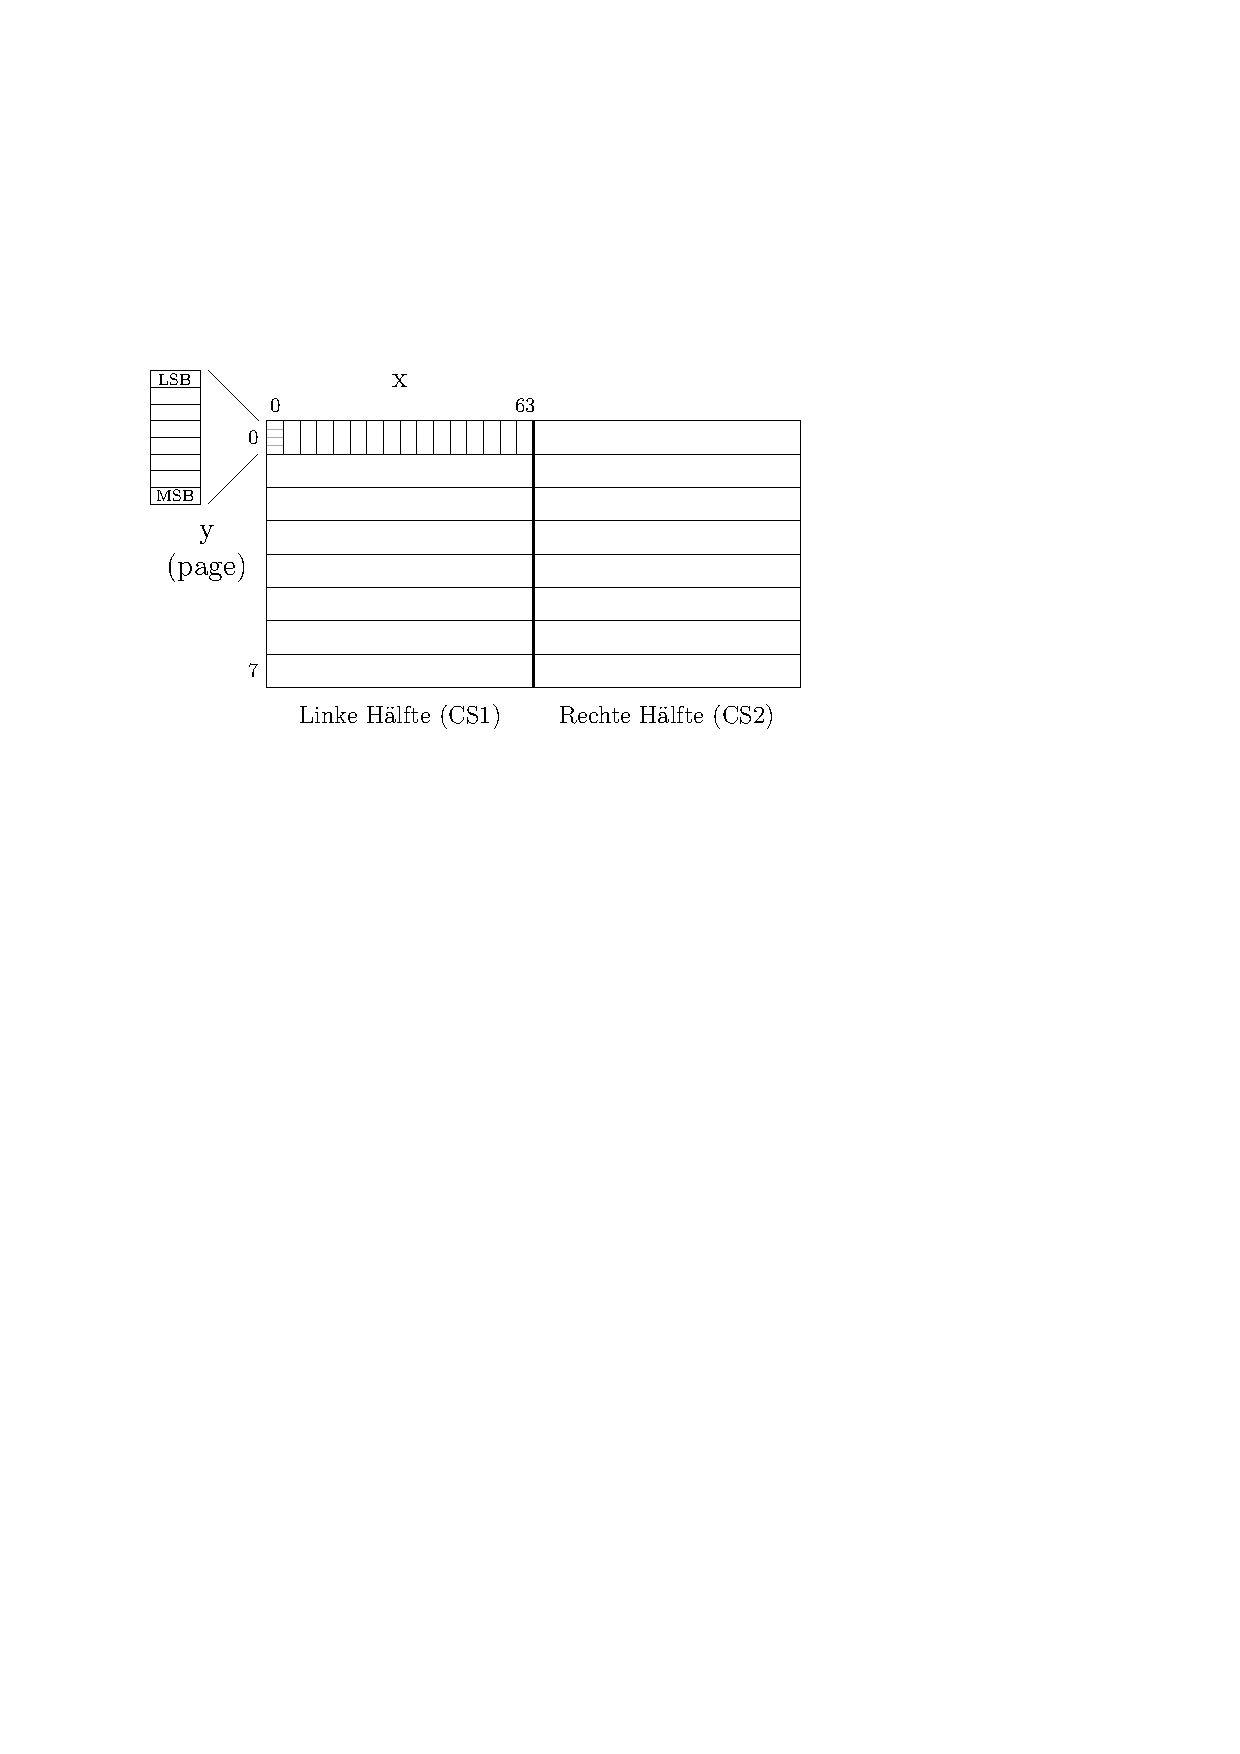
\includegraphics[width=0.6\textwidth]{figures/display_aufbau}
\end{center}

Welche Hälfte einen Befehl verarbeiten soll, wird ausgewählt, indem deren Chip-Select-Signal auf 1 gesetzt wird, das andere auf 0:
\lstinputlisting{problems/listings/display_parts.c}
